\documentclass[a4paper]{article}

% Language and fonts
\usepackage[english]{babel}
\usepackage[utf8x]{inputenc}
\usepackage[T1]{fontenc}

%% Page size setup
\usepackage[a4paper,top=3cm,bottom=2cm,left=3cm,right=3cm,marginparwidth=1.75cm]{geometry}

%% Additional packages
\usepackage{amsmath}
\usepackage{graphicx}
\usepackage{subfigure}
\usepackage[colorinlistoftodos]{todonotes}
\usepackage[colorlinks=true, allcolors=blue]{hyperref}
\usepackage{hyperref}
\usepackage{booktabs}
\usepackage[natbibapa]{apacite}
\usepackage[]{natbib}

%% Setup of Hyperef parameters
\hypersetup{
	pdftitle={Robust estimates for Linear Regression Coefficients},
	pdfauthor={Nicol\'{a}s P\'{e}rez},
	pdfsubject={cool stuff},
	pdfkeywords={Robust, Linear Regression, Coefficients, Betas, Bain},
	bookmarksnumbered=true,     
	bookmarksopen=true,         
	bookmarksopenlevel=1,       
	colorlinks=true,
	citecolor=blue,
	linkcolor=blue,
	urlcolor=blue,                 
	pdfstartview=Fit,           
	pdfpagemode=UseOutlines,      
	pdfpagelayout=SinglePage
}

%% Start doucument
\begin{document}

\begin{center}
\vspace{20mm}
{\Huge Robust Estimates for Linear Regression Coefficients}\\[4mm]

\vspace{40mm}
\textsc{Utrecht University}\\
\vspace{5mm}
{\large Methodology and Statistics for the Behavioural, Biomedical and Social sciences\\
\vspace{30mm}
\textsc{}}\\
\vspace{20mm}

{\Large Research Seminar\\}
\vspace{12mm}

\vspace{6mm}
{\large \textit{Author:}}\\
\vspace{4.5mm}
{\large\textsc{Nicolás Pérez}}\\
(Student number: 5824176)\\
\vspace{6mm}
{\large \textit{Supervisors:}}\\
\vspace{4.5mm}
{\large\textsc{Professor Herbert Hoijtink}}\\
\vspace{4.5mm}

{\large\textsc{\date{\today}}}
\vspace{30mm}


\end{center}

\clearpage

\section{Introduction} \label{introduction}
Multiple linear regression is one of the most used statistical techniques to model the relationship between a dependent variable and predictors. As many other statistical models, linear regression relies on some assumptions; even if the common estimation procedure (OLS) is not distributional dependent, most of the common hypothesis tests and inferences related to it rely on the existence of some statistical distribution in the population (represented by the sampled data). Under ideal conditions, such model assumes independent normally distributed residuals and some degree of correlation of the outcome variable when modeled as a linear combination of the independent variables (amongst other assumptions). A general representation of the linear regression model is:

\begin{equation*}
y_i=\beta_{0}+\beta_{1}X_{1i}+\beta_{2}X_{2i}+...+\beta_{p}X_{pi}+e_i \quad , \quad \text{for } i=1,2...,N \quad ,
\end{equation*}

\noindent
where:
\begin{equation*}
e_i\sim{}N(0,\sigma^{2}).
\end{equation*}

\vspace{3mm}
Several studies have been made regarding the assumptions of the linear regression model and the impact when the data deviates from them. Violations of such assumptions usually imply that the coefficient estimates are wrong; whether because they could be biased or because their standard errors are under/over estimated. For example, as mentioned by (\citeauthor{wilcox2016}, \citeyear{wilcox2016}, p.520-521), outliers presence may not only bias the estimates by shifting the regression line to adjust for the extreme residual value, but they could also imply a smaller standard error of the associated coefficient (given the increase of the sum of squares of the related variable). On the other hand, heteroscedastic residuals do not always affect the estimate value itself (unbiased) but they often lead to a wrong estimation of the standard error of the coefficients (meaning the variance of the estimates is biased).

Robust estimation represents a solution for situations when the data do not fulfill the requirements and assumptions of the underlying model. Many authors have contributed to the topic and even if such tools clearly result in an interesting alternative to traditional approaches, it must be noticed that robust procedures are particular for different models and their assumptions. It is also important to understand that many of the robust methods available today take profit of the development of computational power to provide estimation techniques that might be impossible to solve analytically, but that can easily be approached via computational algorithms. All these factors have contributed to the development of robust estimation, making it a much more popular technique nowadays. 

Despite the fact that robust statistics have been studied in depth and that they are widely available, most of these techniques are still rarely used \citep{wilcox2016}. In this paper, a simulation study was performed to investigate if the robust estimates perform as well as the OLS estimates, in terms of being unbiased and having similar (or not worse) coverage probabilities of the true population parameters. Such analysis is performed when all the assumption of the regression model are met and also when one of the predictors contains outliers. For such purpose, a reference population (sample size, coefficient values, sampling population, etc.) was defined based on situations that are often encountered in the social sciences. Given the importance and variety of robust estimation procedures, we will briefly discuss why the "lmRob" from the "robust" package \citep{robustpackage} is chosen for our analysis and why it is useful when the assumptions of interest (outliers presence and heteroscedasticity) are not met.

In Section \ref{simprocedures} we discuss the simulation procedure for the data of a linear regression model under ideal conditions and we extend the concept to a scenario with presence of outliers. Subsequently, in Section \ref{robustestimation} we make a brief definition of robust estimates and their properties, and how they are related to the estimation technique that we chose for our analysis. Finally, in Section \ref{results} we present the results, comparing OLS estimates and robust estimates in the simulated data and the performance of both techniques.

\section{Simulation Procedure} \label{simprocedures}
\subsection{Method}
To investigate the performance of robust estimates for the linear regression coefficients, we perform a simulation study that allows to evaluate and compare the performance of OLS estimates with what is known as robust MM estimates (Section \ref{robustestimation}). To accomplish this, we simulate a large number of datasets that follow a linear regression model. After this, we estimate the coefficients and their standard error for each dataset (using robust and non-robust regression) in order to compute the coverage probabilities. We expect to find a similar performance on the coverage probabilities in both estimation methods. The detailed design is explained in the next section.  

\subsection{Simulation Design} 
For the simulation, a 1000 datasets are simulated with three different sample sizes, $N=\{25,50,100\}$. Each dataset considers a multiple regression model where 3 independent variables ($X_1, X_2, X_3$) are sampled from a multivariate standard normal distribution:

\begin{equation*}
\left(\begin{array}{c}X_{1i}\\ X_{2i}\\X_{3i}\end{array}\right)\sim N \begin{bmatrix}\left(\begin{array}{c}0\\ 0\\0\end{array}\right), \mathbf{\Sigma} \end{bmatrix}
\end{equation*}

\vspace{2mm}
\noindent
The sampling procedure of the independent variables is done using the "mrvnorm" function from the "MASS" package in R \citep{masslibrary} and receives the desired covariance matrix (also the correlation matrix in this case) of the independent variables as an input; for the purpose of this exercise, no serious multicollinearity is considered and thus the following covariance matrix (\textbf{$\Sigma{}$}) is used:
\[
\mathbf{\Sigma}=
\begin{bmatrix}
1.00 & 0.11 & 0.08 \\
0.11 & 1.00 & 0.14 \\
0.08 & 0.14 & 1.00
\end{bmatrix}
\]

\vspace{1.5mm}
\noindent
Given the sampled values of $X_{1i}$, $X_{2i}$ and $X_{3i}$, the outcome variable is defined by the multiple regression model as:

\begin{equation}
y_i=\beta_{0}+\beta_{1}X_{1i}+\beta_{2}X_{2i}+\beta_{3}X_{3i}+e_i \quad , \quad \text{for } i=1,2...,N \quad ,
\end{equation}

\noindent
where:
\begin{equation*}
e_i\sim{}N(0,\sigma^{2}).
\end{equation*}

\vspace{3mm}
\noindent
In order to be able to sample values of the outcome variable, the values of the coefficients and the residual variance have to be defined. For the case of this simulation, the chosen values for the coefficients are $\beta_0=2$, $\beta_1=3$, $\beta_2=4$, and $\beta_3=5$. Subsequently, the value for the standard deviation of the residuals has to be specified to model the outcome variable. To do so, we control the value of the $R^2$ by setting it to be equal to 0.5, and after this we proceed with the estimation of the residual variance as a function of the already known/set parameters. In simple terms, we want to obtain an expression for $\sigma^2$ that depends on the values of $\beta$'s, \textbf{$\Sigma$} and $R^2$. We begin by expressing the variance of the model as follows:

\begin{equation*}
Var(y)=Var(\beta_{0}+\sum_{j=1}^p\beta_{j}X_{j}+e)
\end{equation*}

\noindent
where $p$ is the total amount of predictors (independent variables) in the model. Such expression can be reordered as:
\begin{equation*}
Var(y)=\sum_{j=1}^p\beta_{j}^2Var(X_{j})+2\sum_{j=1}^p\sum_{k=1}^{j-1}\beta_{j}\beta_{k}Cov(X_{i},X_{j})+\sigma^2.
\end{equation*}

\noindent
Recalling that the $R^2$ can be expressed as the proportion of variance explained by the model over the total variance, we can define
\begin{equation*}
R^2=\frac{\sum_{j=1}^p\beta_{j}^2Var(X_{j})+2\sum_{j=1}^p\sum_{k=1}^{j-1}\beta_{j}\beta_{k}Cov(X_{i},X_{j})}{\sum_{j=1}^p\beta_{j}^2Var(X_{j})+2\sum_{j=1}^p\sum_{k=1}^{j-1}\beta_{j}\beta_{k}Cov(X_{i},X_{j})+\sigma^2}.
\end{equation*}

\vspace{3mm}
\noindent
Rearranging the terms and solving for the variance of the residuals we obtain:

\begin{equation}
\sigma^2=\frac{(1-R^2)}{R^2}\left(\sum_{j=1}^p\beta_{j}^2Var(X_{j})+2\sum_{j=1}^p\sum_{k=1}^{j-1}\beta_{j}\beta_{k}Cov(X_{i},X_{j})\right).
\end{equation}

\vspace{3mm}
\noindent
Using Equation (1) and Equation (2), we can define our regression model as

\begin{equation*}
y_i=2+3X_{1i}+4X_{2i}+5X_{3i}+e_i \quad , \quad \text{for } i=1,2...,N \quad ,
\end{equation*}

\noindent
where:
\begin{equation*}
e_i\sim{}N(0,60.64).
\end{equation*}

\section{Robust Estimation} \label{robustestimation}
Extensive literature exists regarding the definition of robustness in statistics. As mentioned before, these techniques are highly relevant in linear regression models, especially when the sampled data deviates from the "ideal conditions" that are implicitly defined for such model. Some of the most problematic scenarios for linear regression are the presence of outliers and/or heteroscedastic residuals. These situations can potentially lead to biased estimates and over/under estimation of the standard error of the coefficients \citep{wilcox2016}. Robust estimates are known to be a good alternative over OLS when such conditions are present \citep{wilcox2016}.

We start with a simple definition by calling an estimator robust if it's value is unaffected or varies slightly when small changes occur in the distribution of it's input values \citep{wilcox2016}. Further definitions are treated in the literature and the reader can refer to \citet{huber1981} and \citet{wilcox2016}. A more specific definition is often used relating it with two mathematical concepts; Quantitative Robustness and Infinitesimal Robustness (\citeauthor{huber1981}, \citeyear{huber1981}; \citeauthor{ruckstuhl2016}, \citeyear{ruckstuhl2016}; \citeauthor{wilcox2016}, \citeyear{wilcox2016}). In the remaining part of this section we explain the importance of such terms and how they relate with robust estimation in the linear regression context. We also present and explain an existing technique (based on this definition) that allows to obtain robust estimators of the coefficients.

\subsection{Quantitative Robustness}
To define "Quantitative Robustness" we address to the so called breakdown point, which refers to the maximal amount (as a proportion of the total sample size) of inconsistent observations (in our context represented by outliers) that can be added to the actual data before an impossible value for the estimator is obtained (\citeauthor{ruckstuhl2016}, \citeyear{ruckstuhl2016}; \citeauthor{wilcox2016}, \citeyear{wilcox2016}). A classic example to understand the term is given when considering the population mean, which breakdown point is 0; it can be easily proven that if a single (large enough) outlier is added to the data, the mean estimate will result in a complete inaccurate value, and thus the maximum proportion of admitted inconsistent observations is 0. Given the relationship between outliers and the breakdown point, it is reasonable to prefer estimators that achieve a higher value for such measure, since they would be able to handle a larger amount of outliers. It is also important to recall, that theoretically, the maximum breakdown point of an estimator is 0.5; in such case, two different distributions exist in the data and its impossible to determine which one represents the truth population.

\subsection{Infinitesimal Robustness}
"Infinitesimal Robustness" is usually investigated through the influence function as a measure of sensibility on the estimator; in other words, what's the effect of an outlier (also referred as polluted observation $x^*$) on the estimator value. To understand what $x^*$ represents, suppose the following example where $X_{1} = \left\{5,3,7,8,9,11,1,6\right\}$. We define $x^*=33$, which represent a large value that would replace a low observation in $X_1$. Given this, a potential new $X_1$ could be $X_{1} = \left\{5,x^*,7,8,9,11,1,6\right\}= \left\{5,33,7,8,9,11,1,6\right\}$. With this definition, the influence function can be seen as an extension of sensitivity analysis for the estimates (as a function of additional large values of $x^*$) when the sample size goes to infinity (\citeauthor{huber1981}, \citeyear{huber1981}; \citeauthor{ruckstuhl2016}, \citeyear{ruckstuhl2016}; \citeauthor{wilcox2016}, \citeyear{wilcox2016}). Note that the interest for the influence function in robustness does not rely on a specific value as it does for the breakdown point, but on the behaviour of such curve; in particular, whether or not this curve is bounded when the value of the extreme observation (outlier) tends to infinity. When such curve is bounded, we find ourselves in a situation of what is known as "Infinitesimal Robustness". In this case, robust estimators with bounded influence curves are preferred since they are robust to the magnitude of the outliers. For further information, influence functions and its mathematical properties are widely discussed by \citet{huber1981} and \citet{wilcox2016}.

\subsection{MM estimators}
In Section 4, a robust procedure known as MM-estimators is applied to the simulated data. Such procedure was developed with the purpose of designing estimators that have a high breakdown point and a bounded influence curve. However, to get a general idea of what MM-estimators are, we first need to introduce an additional concept: M-Estimators. One of the first approaches to develop robust estimators in the context of linear regression models was studied by \citet{huber1981} and are known as M-estimators. These kind of estimators are based on finding a set of coefficients that minimizes a function (usually denoted by $\rho$) of the residuals ($e_i$) given the observed data. Moreover, they focus on using a "weighting function" that gives smaller importance to extreme or/and unusual observations. The general form of such problem in linear regression can be written as:

\begin{equation*}
\min \sum_{i=1}^{N}\rho(e_i) \qquad \Rightarrow \qquad \frac{\partial}{\partial\beta}\sum_{i=1}^{N}\rho(e_i)=0
\end{equation*}

\noindent
where:

\begin{equation*}
e_i=f(X_{1i},X_{2i},...,X_{pi},y_i,\beta_0,\beta_1,...,\beta_p)
\end{equation*}

\vspace{3mm}
\noindent
From this formal definition it is possible to see that OLS estimates are a specific form of M-estimators, where the chosen function is the squared of the residuals. The M-estimation form for the OLS method can be defined by solving the regression model equation for the residuals
\begin{equation*}
e_i=f(X_{1i},X_{2i},...,X_{pi},Y_i,\beta_0,\beta_1,...,\beta_p)=y_i-(\beta_{0}+\sum_{j=1}^p\beta_{j}X_{j}) \quad , \quad \text{for } i=1,2...,N \quad ,
\end{equation*}

\noindent
and defining the weighting function $\rho(e_i)=e_i^2$, which leads to the common minimization problem of the squared residuals
\begin{equation*}
\min \sum_{i=1}^{N}\rho(e_i)=\sum_{i=1}^{N}(e_i)^2 \quad , \quad \text{for } i=1,2...,N \quad.
\end{equation*}

\vspace{2mm}
\noindent
The most important part of such definition is the dependence of the estimates results on the choice of the weighting function ($\rho$). It is also important to notice that depending on the complexity of the chosen function, the solution for such problem might also be more complicated. Many studies have been done regarding which functions should be used to obtain solutions that provide good results in terms of robustness (\citeauthor{wilcox2016}, \citeyear{wilcox2016}; \citeauthor{huber1981}, \citeyear{huber1981}). 

Even if M-estimators sound conceptually appropriate, it can be proven that M-estimates have a breakdown point of 0, meaning that the addition of a very large outlier could result on a completely wrong estimation of the parameters of interest (\citeauthor{ruckstuhl2016}, \citeyear{ruckstuhl2016}; \citeauthor{wilcox2016}, \citeyear{wilcox2016}).
To address this issue, \citet{yohai1987} proposed a different approach called MM-estimators. These estimators are based on the concept of M-estimators but are built departing from the principle of obtaining estimators which breakdown point is maximal (i.e. 0.5) and that are highly efficient (in the context of relative variance - Cramer Rao Bound). MM-estimators are obtained by an iterative process that starts by finding an estimator with maximal breakdown point (several options are available to accomplish this). After this, the M-estimation procedure is used to minimize the scaled residuals through the so called "loss function" and the estimation of the coefficients. In this sense, MM-estimators not only accomplish the desired conditions of a high breakdown point and a bounded influence curve but they are also more efficient than other robust estimators. For detailed information about the algorithm, how it works and its properties, reader may refer to \citet{yohai1987}.


\subsection{Robust Linear Regression in R} \label{robustregression}
Different packages are available to perform robust analysis in R \citep{rsoftware} such as the "rlm", "lmrob"  and "lmRob" in the "MASS" \citep{masslibrary}, "robustbase" \citep{robustbase} and "robust" \citep{robustpackage} packages respectively (amongst others).  For this simulation, the mentioned packages were tested and their documentation was reviewed, which lead to choosing the "robust" package. The main reasons to choose it were that the original author of the MM-estimators is part of the authors of such package and also because of its time efficiency. 

\subsubsection{Coefficients estimation}
Using the model specified in Section \ref{simprocedures}, OLS regression and robust regression were performed for every set of datasets under the three given sample sizes, and the estimates of the coefficients and their standard deviation were stored. Given that the "true population" parameter values of the coefficients are known, coverage probabilities can be computed by counting the amount of cases where the true parameter value lays in the confidence interval obtained by the model estimation. The coverage probabilities are computed for the two regression methods on the four coefficients under the three defined sample sizes (See Table \ref{table1}).  It is known that OLS estimates follow a t-distribution with $N-p$ degrees of freedom. It can also be shown that MM-estimators for regression coefficients follow the same distribution (asymptomatically). Figure \ref{Figure1} shows the distributions of the 4 coefficients under the OLS and robust estimation. 

\section{Results} \label{results}
The following table presents the coverages probabilities for the regression coefficients under the estimation procedures.

\begin{table}[!h]
	\centering
	\caption{Coverage probabilities of the regression coefficients - Perfect conditions}
	\vspace{1mm}
	\label{table1}
	\begin{tabular}{@{}ccccccccc@{}}
		\toprule
		& \multicolumn{2}{c}{N=25} & \textit{} & \multicolumn{2}{c}{N=50} & \textit{} & \multicolumn{2}{c}{N=100} \\ \midrule
		& OLS       & Rob. Reg.    & \textit{} & OLS       & Rob. Reg.    & \textit{} & OLS       & Rob. Reg.     \\
		$\mathbf{\beta_{0}}$ & 0.949                 & 0.961                       &           & 0.942                 & 0.970                       &           & 0.948                 & 0.968                       \\
		$\mathbf{\beta_{1}}$ & 0.958                & 0.962                       &           & 0.944                 & 0.972                       &           & 0.958                 & 0.968                       \\
		$\mathbf{\beta_{2}}$ & 0.939                 & 0.946                       &           & 0.956                 & 0.979                       &           & 0.940                  & 0.957                       \\
		$\mathbf{\beta_{3}}$ & 0.944                 & 0.949                       &           & 0.958                 & 0.977                       &           & 0.948                 & 0.964      \\   
		\bottomrule         
	\end{tabular}
\end{table}


\noindent
It can be seen (Table \ref{table1}) that coverage probabilities are almost equivalent for all coefficients with the two estimation methods independently of the sample size. The most interesting result is that even for small samples, both procedures perform equally well, allowing the researcher to choose which one to use under given circumstances. However, it results natural to think that a specific outlier (same in both cases) will have a more drastic effect in a smaller dataset, indicating that for very small samples robust estimates perform probably better. The following table summarizes the same results when replacing a value of $X_{1i}$ (randomly picked from the bottom 10\% percentile of $X_1$) by an outlier. Outliers were generated by randomly sampling (uniformly) from the following interval

\vspace{3mm}
\begin{equation*}
X_{1}^{out}=\left[X_{1,Q_{0.75}}+1.5IQR\; ; \; X_{1,Q_{0.75}}+3IQR \right]
\end{equation*}

\begin{table}[!h]
	\centering
	\caption{Coverage probabilities of the regression coefficients - Additional outlier}
	\vspace{1mm}
	\label{table2}
	\begin{tabular}{@{}ccccccccc@{}}
		\toprule
		& \multicolumn{2}{c}{N=25} & \textit{} & \multicolumn{2}{c}{N=50} & \textit{} & \multicolumn{2}{c}{N=100} \\ \midrule
		& OLS       & Rob. Reg.    & \textit{} & OLS       & Rob. Reg.    & \textit{} & OLS       & Rob. Reg.     \\
		$\mathbf{\beta_{0}}$ & 0.951                 & 0.959                       &           & 0.953                 & 0.977                       &           & 0.944                 & 0.953                       \\
		$\mathbf{\beta_{1}}$ & 0.395                & 0.941                       &           & 0.414                 & 0.967                       &           & 0.519                 & 0.967                       \\
		$\mathbf{\beta_{2}}$ & 0.935                 & 0.941                       &           & 0.946                 & 0.973                       &           & 0.946                  & 0.965                       \\
		$\mathbf{\beta_{3}}$ & 0.939                 & 0.943                       &           & 0.959                 & 0.981                       &           & 0.933                 & 0.954   \\         
		\bottomrule      
	\end{tabular}
\end{table}

\noindent
Table \ref{table2} shows that the coverage probabilities of the regression coefficient with the outlier is drastically affected under OLS and unaffected with robust estimates. We also see that as the sample size increases, the coverage probability for such coefficient improves.

\section{Discussion}
The aim of the simulation study was to evaluate the performance of robust estimates for linear regression coefficients and compare them to the OLS estimates that are frequently used. Results show that for different sample sizes, robust estimates and OLS estimates perform equally and give similar results when all the assumptions of the linear regression model are met. On the other hand, when outliers are present in the data, robust estimates show their superiority and should be preferred over OLS. Moreover, the research question can be now expanded to establish a statistical criterion to chose which kind of estimates should be used under specific conditions of outliers presence and heteroscedasticity. 

\newpage
\bibliographystyle{apacite}
\bibliography{bibliography}

\newpage

\section*{Figures} \label{Figures}

\vspace{22mm}
\begin{figure}[h]
	\begin{center}
		\resizebox{\textwidth}{!}{ %RESIZING RELATIVE TO HE WIDTH
			\subfigure[Histogram $\beta_{0}$]{
				\label{a:histogram}
				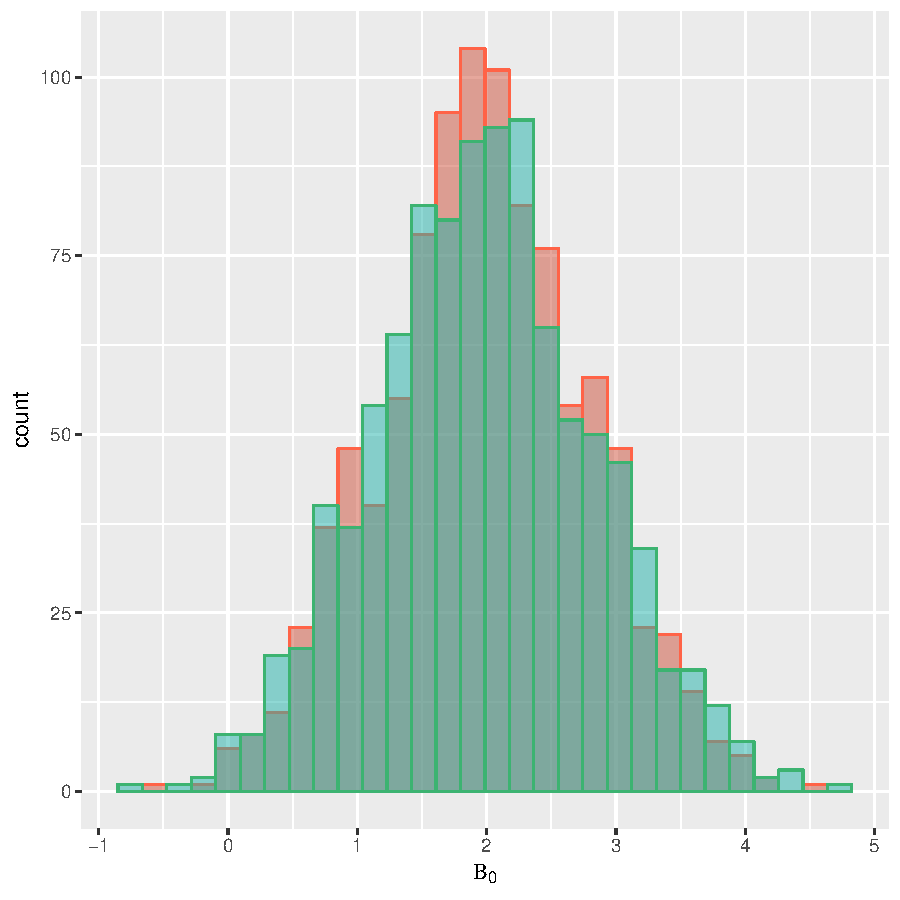
\includegraphics[scale=.5]{beta0ideal.pdf}
			}
			\subfigure[Histogram $\beta_{1}$]{
				\label{b:Densityplot}
				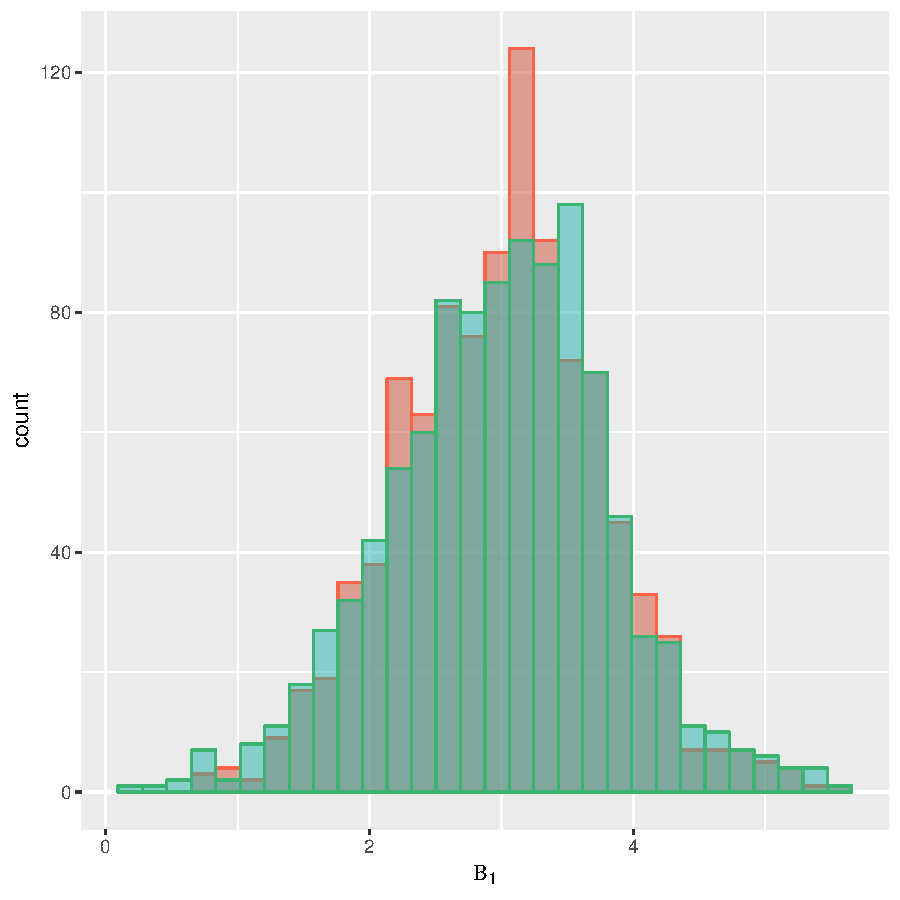
\includegraphics[scale=.5]{beta1ideal.pdf}
			}
		}\\ 	%  ------- End of the first row ----------------------%
		\resizebox{\textwidth}{!}{
			\subfigure[Histogram $\beta_{2}$]{
				\label{c:Stripplot}
				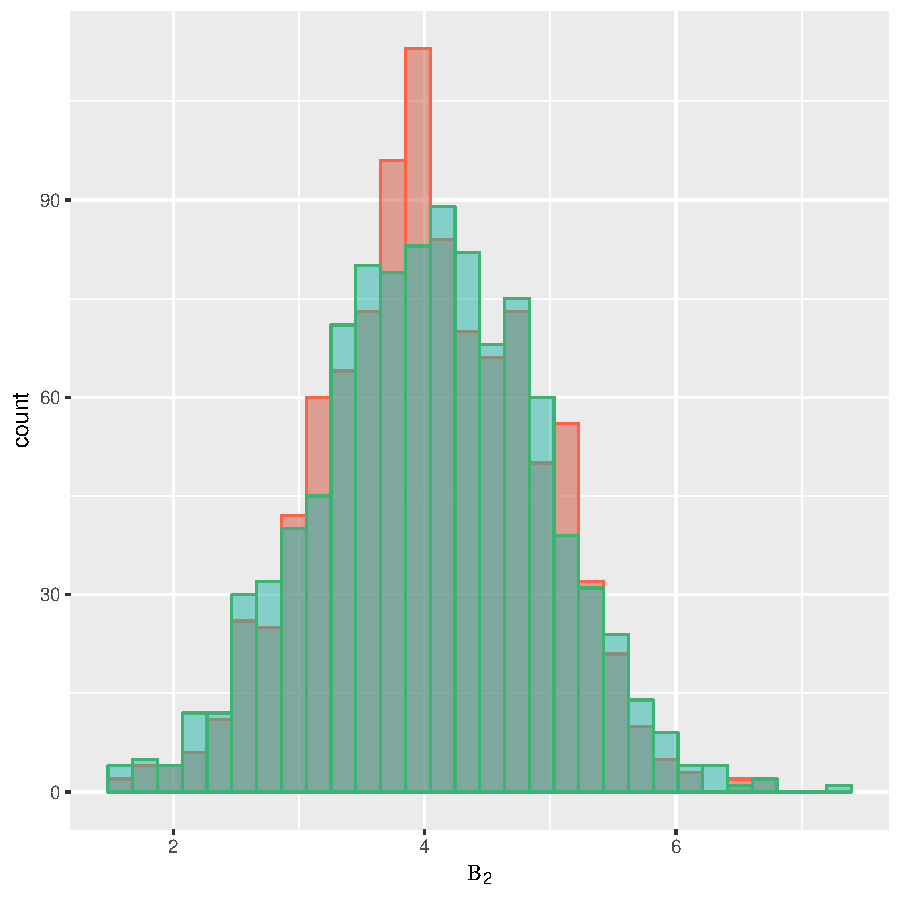
\includegraphics[scale=.5]{beta2ideal.pdf}
			}
			\subfigure[Histogram $\beta_{3}$]{%
				\label{d:Boxplot}
				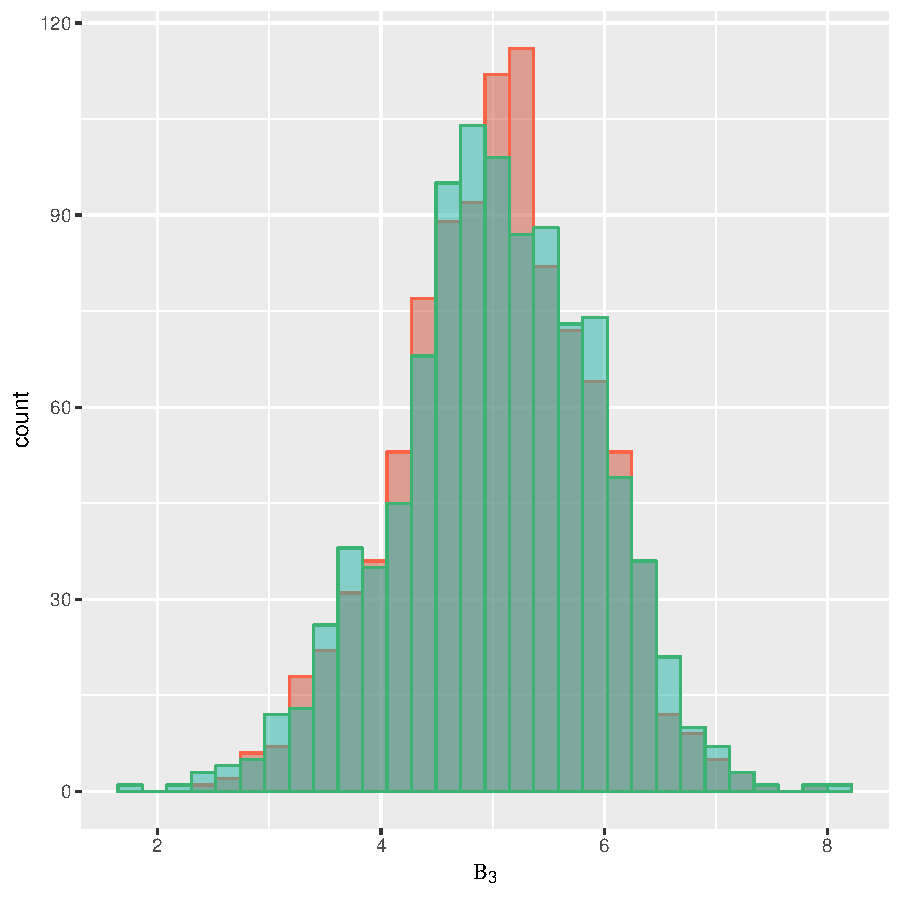
\includegraphics[scale=.5]{beta3ideal.pdf}
			}
		}
	\end{center}
	\caption{Histograms of the regression coefficients under the two regression methods with ideal conditions (N=100). Light-red bars correspond to OLS estimates and green bars to robust estimates.}
	\label{Figure1}
\end{figure}

\newpage

\begin{figure}[p]
	\begin{center}
		\resizebox{\textwidth}{!}{ %RESIZING RELATIVE TO HE WIDTH
			\subfigure[Histogram $\beta_{0}$]{
				\label{a:histogram}
				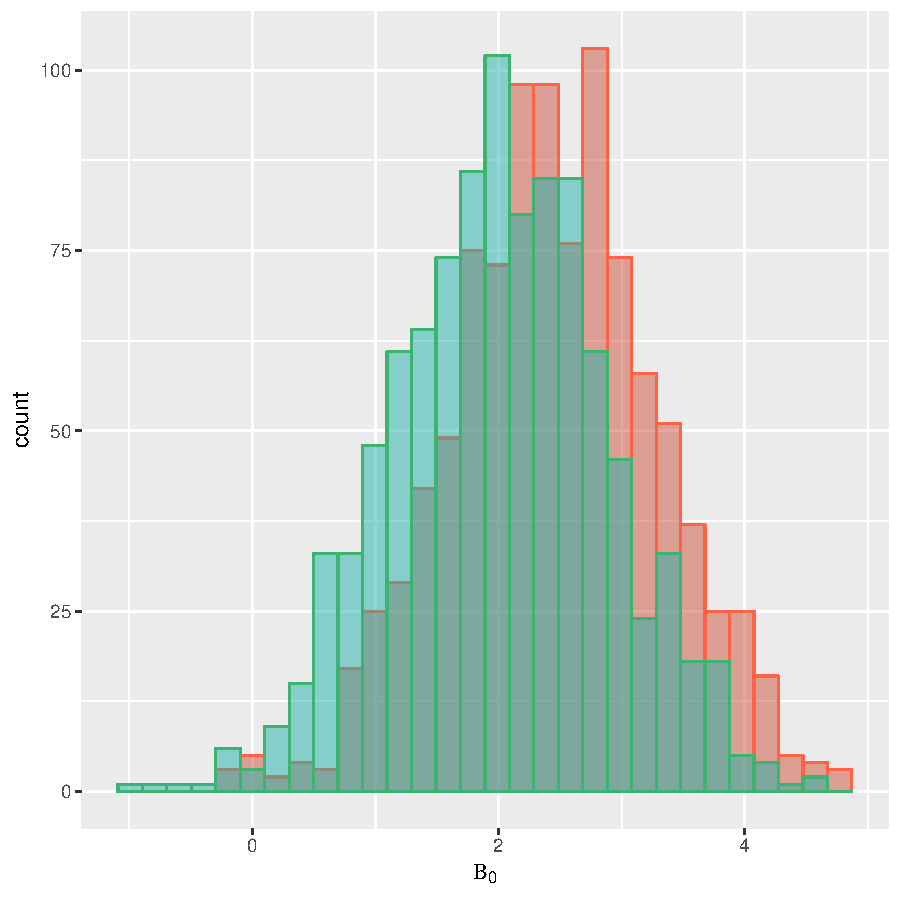
\includegraphics[scale=.5]{beta0outliers.pdf}
			}
			\subfigure[Histogram $\beta_{1}$]{
				\label{b:Densityplot}
				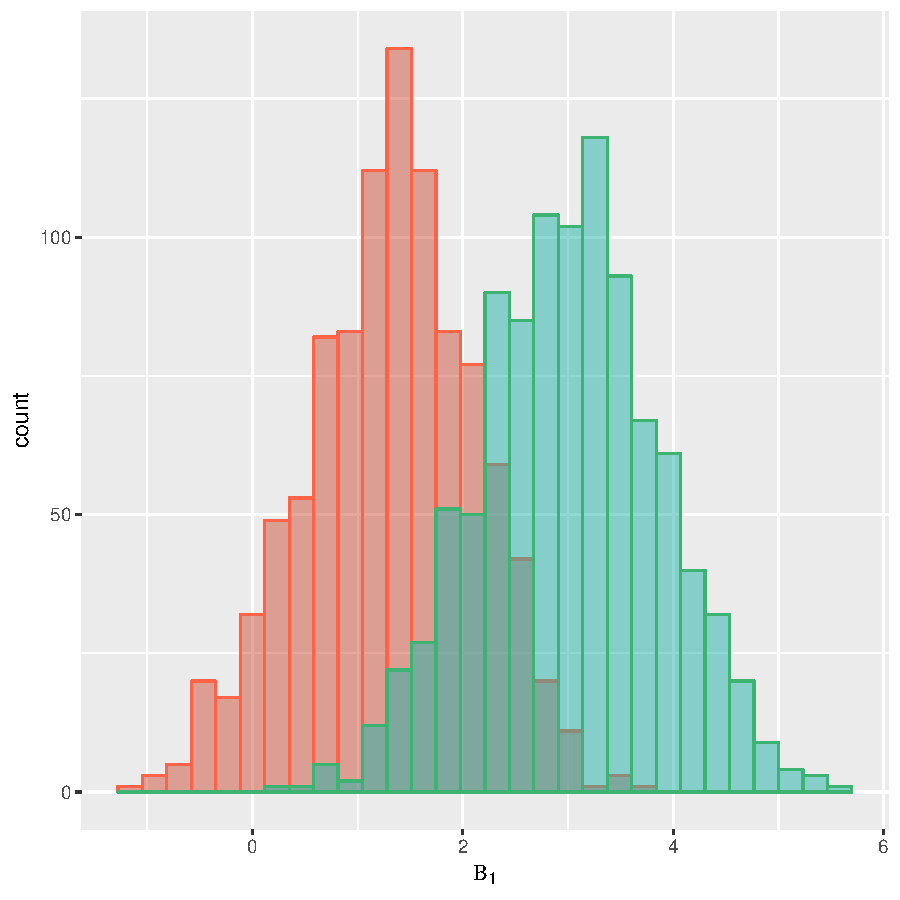
\includegraphics[scale=.5]{beta1outliers.pdf}
			}
		}\\ 	%  ------- End of the first row ----------------------%
		\resizebox{\textwidth}{!}{
			\subfigure[Histogram $\beta_{2}$]{
				\label{c:Stripplot}
				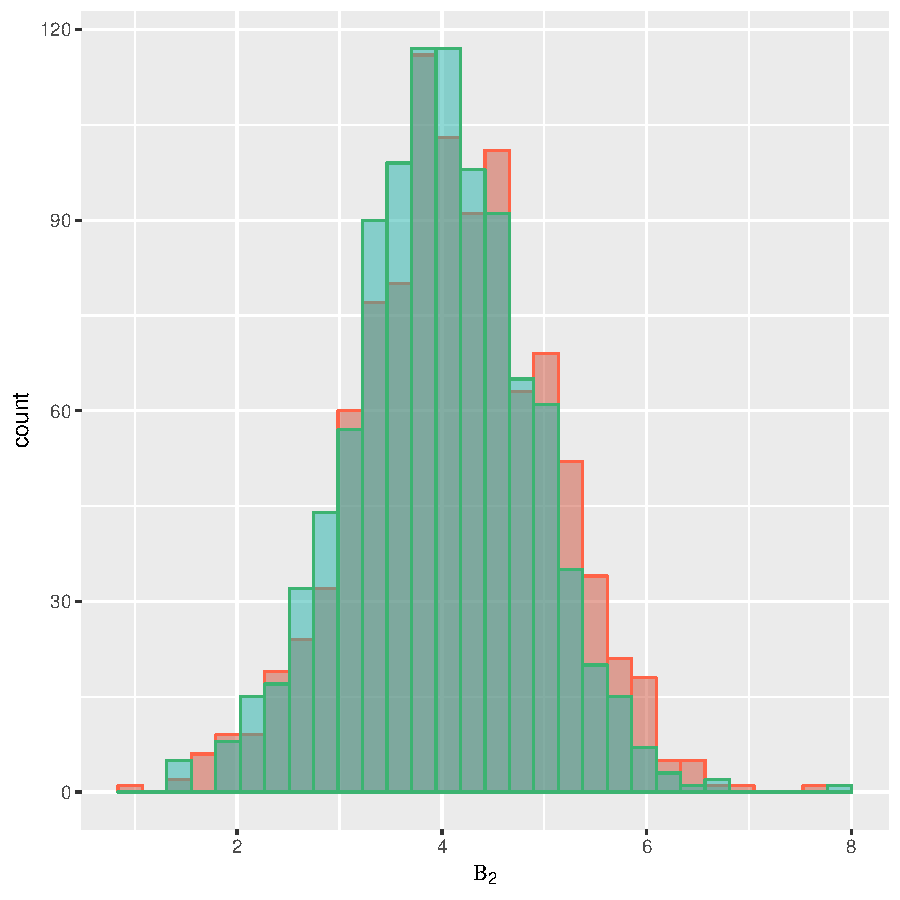
\includegraphics[scale=.5]{beta2outliers.pdf}
			}
			\subfigure[Histogram $\beta_{3}$]{%
				\label{d:Boxplot}
				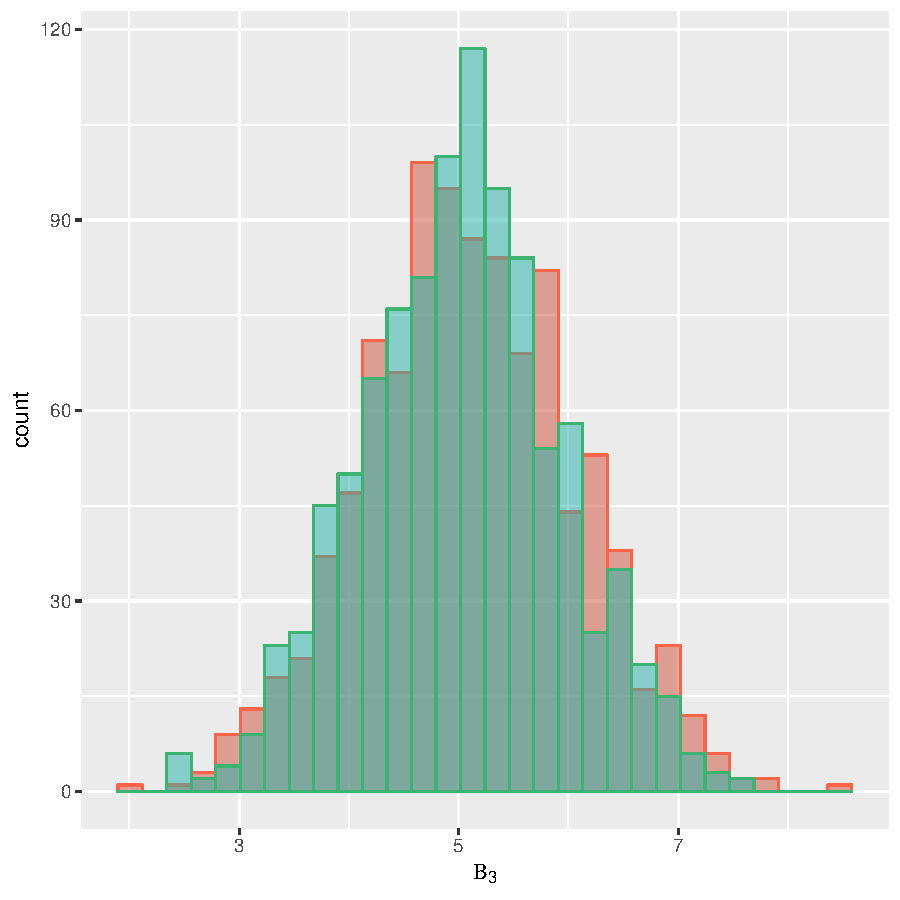
\includegraphics[scale=.5]{beta3outliers.pdf}
			}
		}
	\end{center}
	\caption{Histograms of the regression coefficients under the two regression methods with presence of outliers (N=100). Light-red bars correspond to OLS estimates and green bars to robust estimates.}
	\label{Figure2}
\end{figure}



\end{document}